\documentclass[main.tex]{subfiles}
\begin{document}
\newpage
\section{Telegrafenrauschen in Samarium-Erbium-Ferrit}

\todo{in allen plots die normierte Magnetisierung verwenden}

\begin{figure}[h]
    \centering
    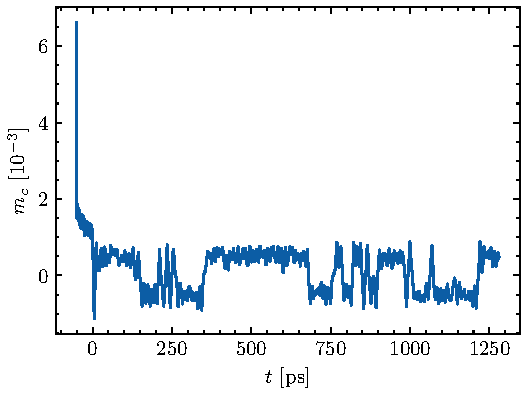
\includegraphics{bilder/plots/theo-vis/example-telegraph-sim.pdf}
    \caption{Einzelne Simulationskurve von \(mu_c\) bei \SI{300}{\kelvin}}\label{fig:bsp-run}
\end{figure}

% \todo{Einzelne Simulationskurve mit Einschwingvorgang}

\subsection{Extraktion des Telegrafenrauschens}

\begin{figure}[h]
    \centering
    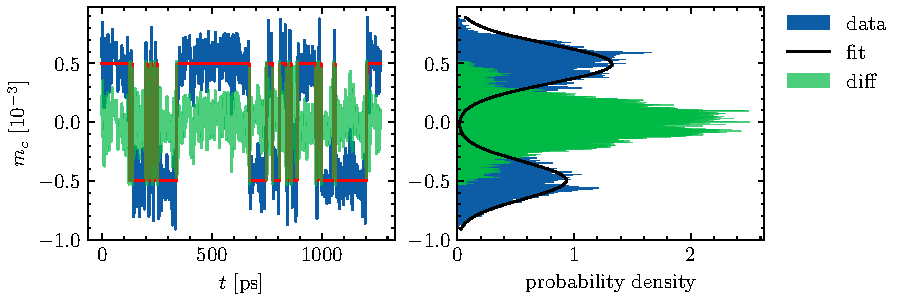
\includegraphics{bilder/plots/Bz_0mT/mc_fit_hist_part2_26.03meV.pdf}
    \caption{Extraktion aus \SI{1,2}{\nano\s}\todo{Andere Farbe für fit und extrahiertes Telegrafenrauschen}}\label{fig:Extraktion-ausschnitt}
\end{figure}

\todo{Gauß vs. Lorenzverteilung zum Fitten?}
% \todo{vergleich mit kmeans?}

\todo{erklärung warum verschiedene Runs einfach hintereinander hängen geht}

\subsection*{Dominanz des Telegrafenrauschens}

\begin{figure}[H]
    \centering
    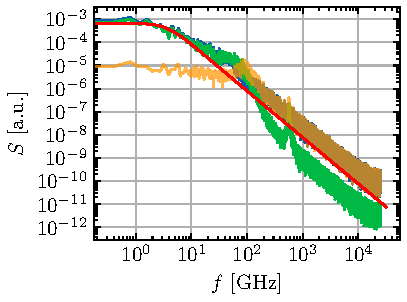
\includegraphics{bilder/plots/Bz_0mT/spectral_power_densities_26.03meV.pdf}
    \caption{Spektrale Leistungsdichten von ursprünglichem und bereinigtem Telegrafenrauschen und Differenz. Simulation bei \SI{26.04}{\milli\electronvolt} ohne externes Magnetfeld.}\label{fig:spds}
\end{figure}

\begin{figure}[H]
    \centering
    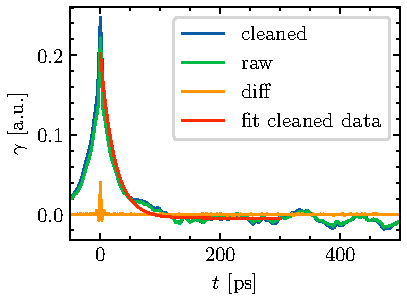
\includegraphics{bilder/plots/Bz_0mT/autocorr_26.03meV.pdf}
    \caption{vergleich Autokorrelation, von ursprünglichem und bereinigtem Telegrafenrauschen und Differenz. Simulation bei \SI{26.04}{\milli\electronvolt} ohne externes Magnetfeld.}\label{fig:autocorr}
\end{figure}

\subsection{Simulation ohne externes Magnetfeld}
\todo{Anderer Titel? Variation der Temperatur}
\subsubsection{In der Zeitdomäne}

\todo{ist es wirklich eine Wahrscheinlichkeitsdichte?}

\begin{figure}[H]
    \centering
    \subcaptionbox{bereich mit sichtbarem TGR\label{fig:temp-hist-tg}}{    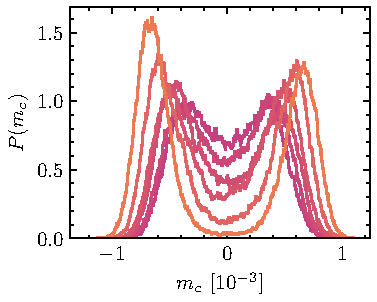
\includegraphics{bilder/plots/temp_comparison_long/mc_hist_tgr.pdf}}
    \subcaptionbox{long \label{fig:temp-hist-long}}{    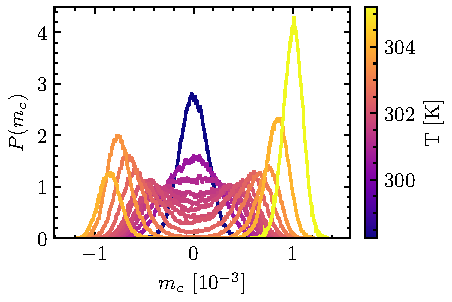
\includegraphics{bilder/plots/temp_comparison_long/mc_hist.pdf}}
    \caption{temp hist\todo{gleiche colormap und nebeneinander}}\label{fig:temp-hist}    
\end{figure}

\begin{figure}[H]
    \centering
    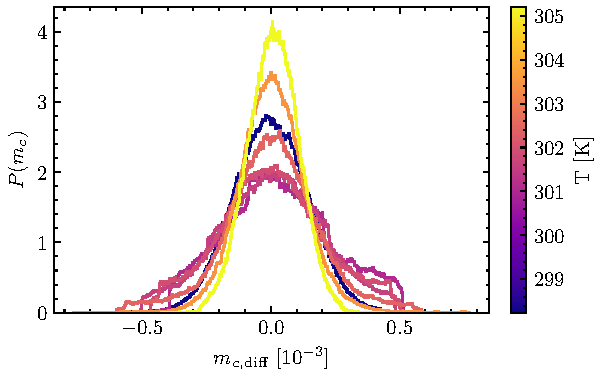
\includegraphics{bilder/plots/temp_comparison_long/mc_diff_hist.pdf}
    \caption{temp diff hist}\label{fig:temp-diff-hist}    
\end{figure}

\begin{figure}[H]
    \centering
    \subcaptionbox{scatter\label{fig:temp-switch-count-scatter}}{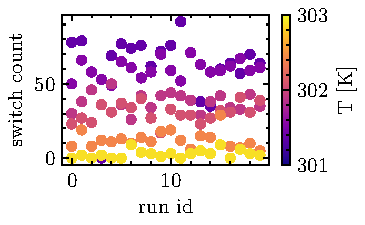
\includegraphics{bilder/plots/temp_comparison/switch_count_scatter.pdf}}
    \subcaptionbox{violin\label{fig:temp-switch-count-violin}}{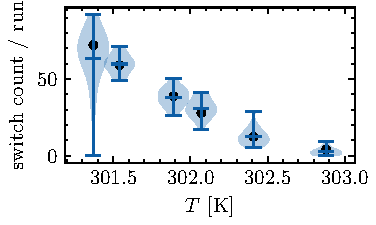
\includegraphics{bilder/plots/temp_comparison/switch_count_violin.pdf}}
    \caption{temp switch count}\label{fig:temp-switch-count}
\end{figure}

\begin{figure}[H]
    \centering
    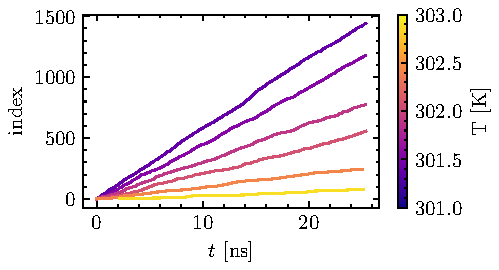
\includegraphics{bilder/plots/temp_comparison/switch_events.pdf}
    \caption{time of switch event}\label{fig:switch-events}
\end{figure}

\begin{figure}[H]
    \centering
    \subcaptionbox{scatter\label{fig:temp-up-percentage-scatter}}{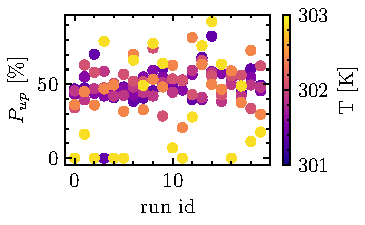
\includegraphics{bilder/plots/temp_comparison/up_percentage_scatter.pdf}}
    \subcaptionbox{violin\label{fig:temp-up-percentage-violin}}{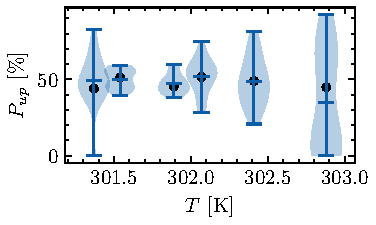
\includegraphics{bilder/plots/temp_comparison/up_percentage_violin.pdf}}
    \caption{temp up percentage}\label{fig:temp-up-percentage}
\end{figure}

\subsubsection{In der Frequenzdomäne}

\begin{figure}[H]
    \centering
    \subcaptionbox{source \label{fig:temp-spd-source}}{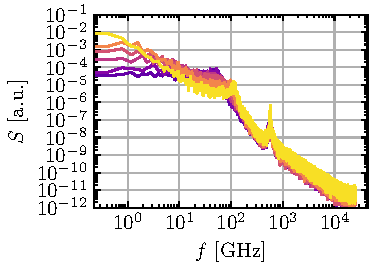
\includegraphics{bilder/plots/temp_comparison/spectral_power_density.pdf}}
    \subcaptionbox{clean \label{fig:temp-spd-clean}}{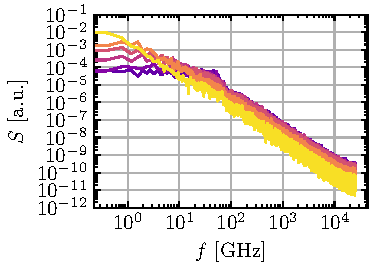
\includegraphics{bilder/plots/temp_comparison/spectral_power_density_cleaned.pdf}}
    \subcaptionbox{diff\label{fig:temp-spd-diff}}{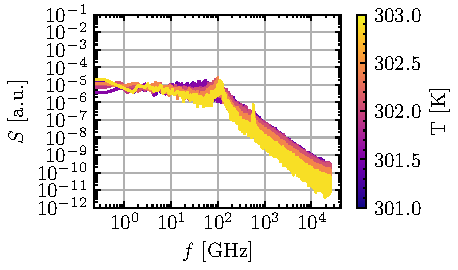
\includegraphics{bilder/plots/temp_comparison/spectral_power_density_diff.pdf}}
    \caption{temp spectral power densities\todo{nur eine colorbar?}}\label{fig:temp-spd}
\end{figure}


\begin{figure}[H]
    \centering
    % \subcaptionbox{source \label{fig:temp-autocorr-source}}{\includegraphics{bilder/plots/temp_comparison/autocorrelation.pdf}}
    \subcaptionbox{clean \label{fig:temp-autocorr-clean}}{\includegraphics{bilder/plots/temp_comparison/autocorrelation_cleaned.pdf}}
    \subcaptionbox{diff\label{fig:temp-autocorr-diff}}{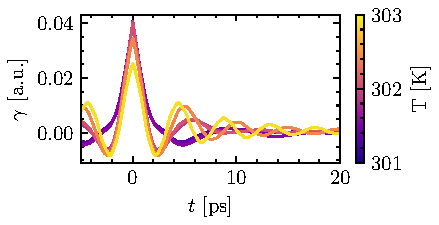
\includegraphics{bilder/plots/temp_comparison/autocorrelation_diff.pdf}}
    \caption{temp autocorrelations}\label{fig:temp-autocorr}
\end{figure}


\todo{Berechnung MDT aus Autokorrelation}

\begin{figure}[H]
    \centering
    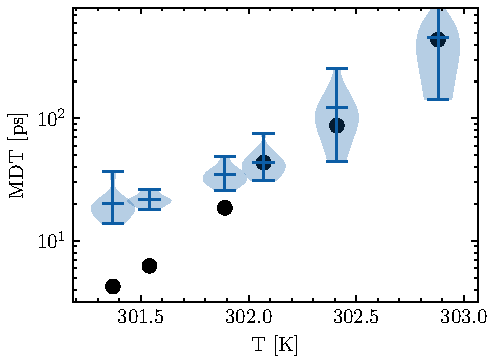
\includegraphics{bilder/plots/temp_comparison/mean_dwell_time_comparison.pdf}
    \caption{temp mean dwell time comparison}\label{fig:temp-mdt-comp}
\end{figure}

\begin{figure}[H]
    \centering
    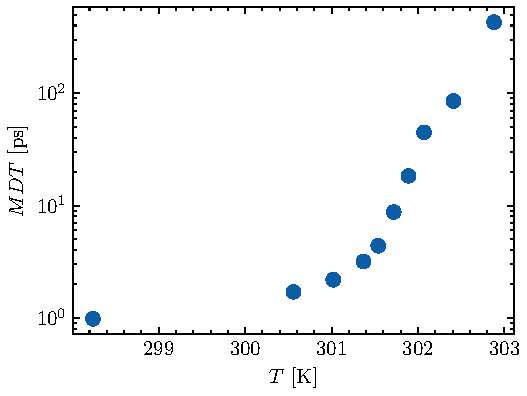
\includegraphics{bilder/plots/temp_comparison_long/mean_dwell_time.pdf}
    \caption{temp mean dwell time long}\label{fig:temp-mdt-long}
\end{figure}


\begin{figure}[H]
    \centering
    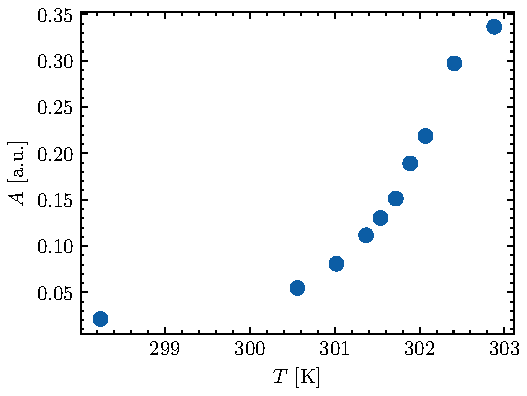
\includegraphics{bilder/plots/temp_comparison_long/rauschamplitude.pdf}
    \caption{temp autocorrelation amplitude (Rauschamplitude)}\label{fig:temp-autocorr-amplitude}
\end{figure}

\subsection{Simulation mit externem Magnetfeld}

\begin{figure}[H]
    \centering
    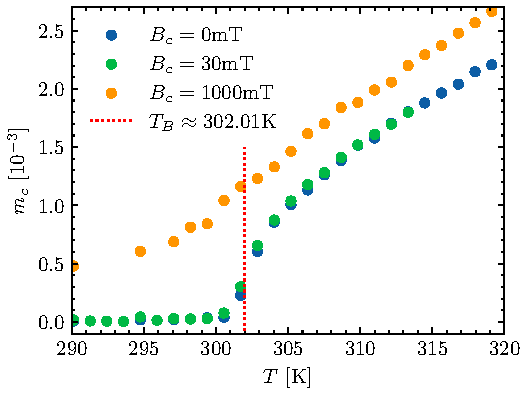
\includegraphics{bilder/plots/Bz_comparison/critical_temperature.pdf}
    \caption{Bz critical temperature \todo{use Kelvin}}\label{fig:bz-crit-temp}
\end{figure}

\todo{Einfluss Vorzeichenumkehr Bz}

\subsubsection{In der Zeitdomäne}

\todo{ist es wirklich eine Wahrscheinlichkeitsdichte?}

\begin{figure}[H]
    \centering
    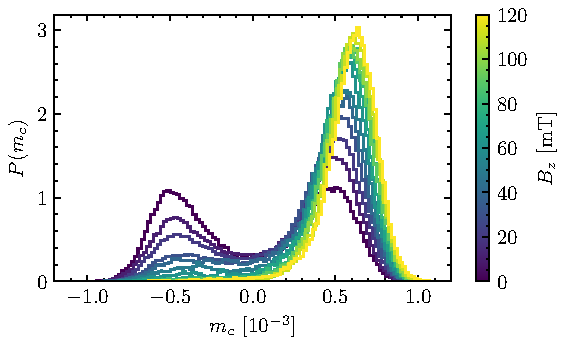
\includegraphics{bilder/plots/max_Bz/mc_hist.pdf}
    \caption{b hist}\label{fig:b-hist}    
\end{figure}

\begin{figure}[H]
    \centering
    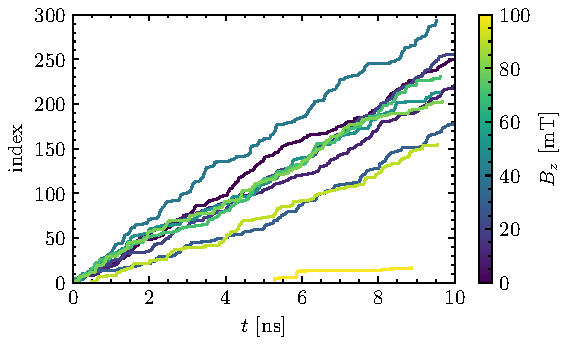
\includegraphics{bilder/plots/max_Bz/switch_events.pdf}
    \caption{time of switch event\todo{größerer Ausschnitt}}\label{fig:bz-switch-events}   
\end{figure}


\begin{figure}[H]
    \centering
    \subcaptionbox{b up percentage violin\label{fig:bz-up-percentage-violin}}{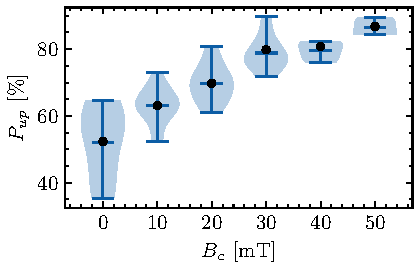
\includegraphics{bilder/plots/max_Bz/up_percentage_violin.pdf}}
    \subcaptionbox{b state times comp\label{fig:bz-state-times-comp}}{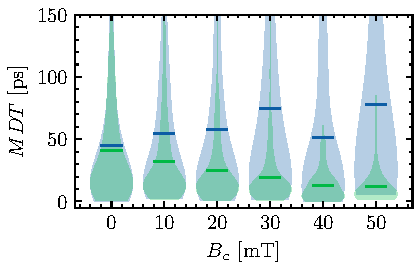
\includegraphics{bilder/plots/max_Bz/state_times_comp.pdf}}
    \caption{b up percentage}\label{fig:bz-violin}
\end{figure}

\subsubsection{In der Frequenzdomäne}


\begin{figure}[H]
    \centering
    \subcaptionbox{source\label{fig:bz-spd-source}}{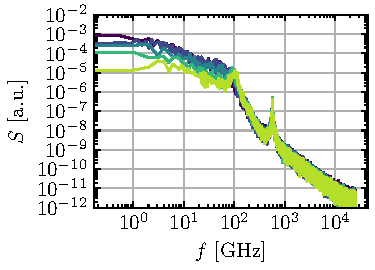
\includegraphics{bilder/plots/max_Bz/spectral_power_density.pdf}}
    \subcaptionbox{clean\label{fig:bz-spd-clean}}{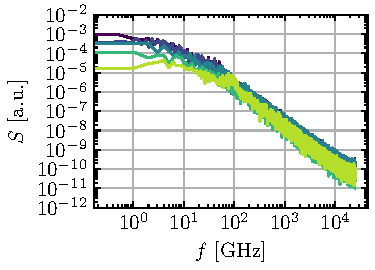
\includegraphics{bilder/plots/max_Bz/spectral_power_density_cleaned.pdf}}
    \subcaptionbox{diff\label{fig:bz-spd-diff}}{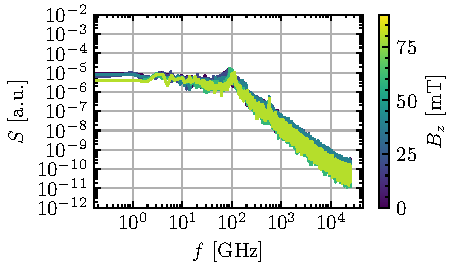
\includegraphics{bilder/plots/max_Bz/spectral_power_density_diff.pdf}}
    \caption{Bz spectral power densities \todo{nur eine colorbar. plots etwas größer}}\label{fig:bz-spd}
\end{figure}


\begin{figure}[H]
    \centering
    \subcaptionbox{source \label{fig:bz-autocorr-source}}{\includegraphics{bilder/plots/max_Bz/autocorrelation.pdf}}
    \subcaptionbox{clean \label{fig:bz-autocorr-clean}}{\includegraphics{bilder/plots/max_Bz/autocorrelation_cleaned.pdf}}
    \subcaptionbox{diff\label{fig:bz-autocorr-diff}}{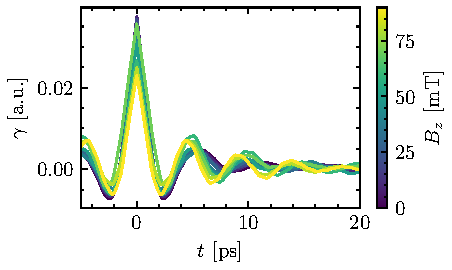
\includegraphics{bilder/plots/max_Bz/autocorrelation_diff.pdf}}
    \caption{Bz autocorrelations \todo{nur eine colorbar. plots etwas größer}}\label{fig:bz-autocorr}
\end{figure}

\todo{Die Mean Dwell time ist nicht aus der Autokorrelation Bestimmbar (Mittlere Mean Dwell time)}

\begin{figure}[H]
    \centering
    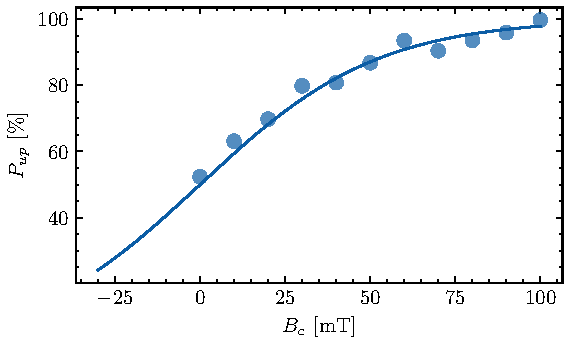
\includegraphics{bilder/plots/max_Bz/up_percentage_fit.pdf}
    \caption{b up percentage sigmoid fit \todo{quelle der Datenpunkte}}\label{fig:bz-up-percentage}
\end{figure}

\begin{figure}[H]
    \centering
    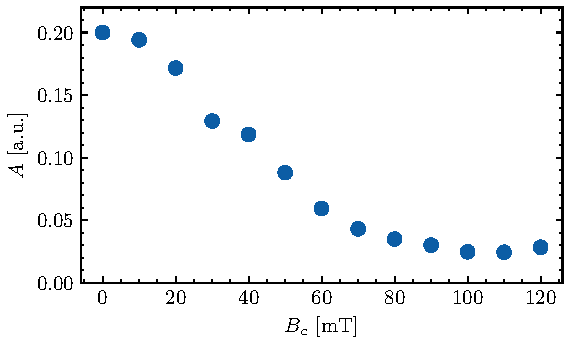
\includegraphics{bilder/plots/max_Bz/rauschamplitude.pdf}
    \caption{Bz rauschamplitude \todo{was bedeutet das?}}\label{fig:bz-rauschampl}
\end{figure}


% bibliography (temporary)
% \bibliography{literatur} \todo{comment out before compiling main.tex}

\end{document}